\chapter{Benchmark}
\label{chap:benchmark}

The main aim of this thesis is to methodically examine the appearance phenomena that are frequently appearing in our day-to-day life but for some reason are still rarely implemented in the modern renderers. However, in the past decade, the interest in the physically realistic renders has grown significantly and the implementations for these phenomena have been introduced. As they are still being consistently improved and integrated into the conventional rendering systems, it is necessary to have a testing suite which would properly evaluate their accuracy.

We propose a testing suite that contains a minimum number of test scenes which maximally exercise these implementations and an equivalent number of the reference images that, to our best knowledge, we consider to be the ground truth. These are encapsulated in an automated workflow, which runs the tests with a single command and shows the results in form of a website. The suite also contains data such as code snippets that should simplify the replication process of these implementations so that they can be easily integrated into any standard renderer.

The benchmark follows a few basic principles:

\begin{description}
	\item[Easy to use] The benchmark should provide a user-friendly environment that is comprehensible for an average developer or tester of the rendering features. Therefore, the whole suite is written in Python3 as it is currently one of the most popular scripting languages, it does not need to be compiled and is cross-platform. It also provides CLI command options that are invoke-able via python command.
	\item[Modularity] Each part of the benchmark should be adjustable without the need to heavily modify the other parts. For example, if a new CLI option is to be added, you only need to change the \texttt{/src/arg\_parser.py} file.
	\item[Extensibility] It should be simple enough to extend the capabilities of the benchmark, such as adding new scenes, test case scenarios, or even renderers. For example, you don't have to modify any code if you want to add a new scene --- there are structures prepared for this scenario which simply need to be filled.
	\item[Simplicity] The scenes are straightforward, containing only basic and portable geometry, light sources, and cameras. This brings two large advantages --- it is fairly easy to replicate them for different renderers and they are simple enough to understand the purpose of each element they contain. Along with the thorough comments, anyone with the basic knowledge acquired in the previous chapters of this thesis should comprehend their meaning.
	\item[Standalone] The benchmark should contain all the data that the potential user would need to properly run or generally use the testing suite. For example, the geometry that is included in the scenes can be found in the \texttt{/data/common/} folder.
\end{description}

\section{Framework}

First of all, we take a look into the framework of the benchmark suite and its structure. The file organization is demonstrated in \autoref{fig:framework} and the following sections describe each major subsection of it.

\begin{figure}
	\centering
	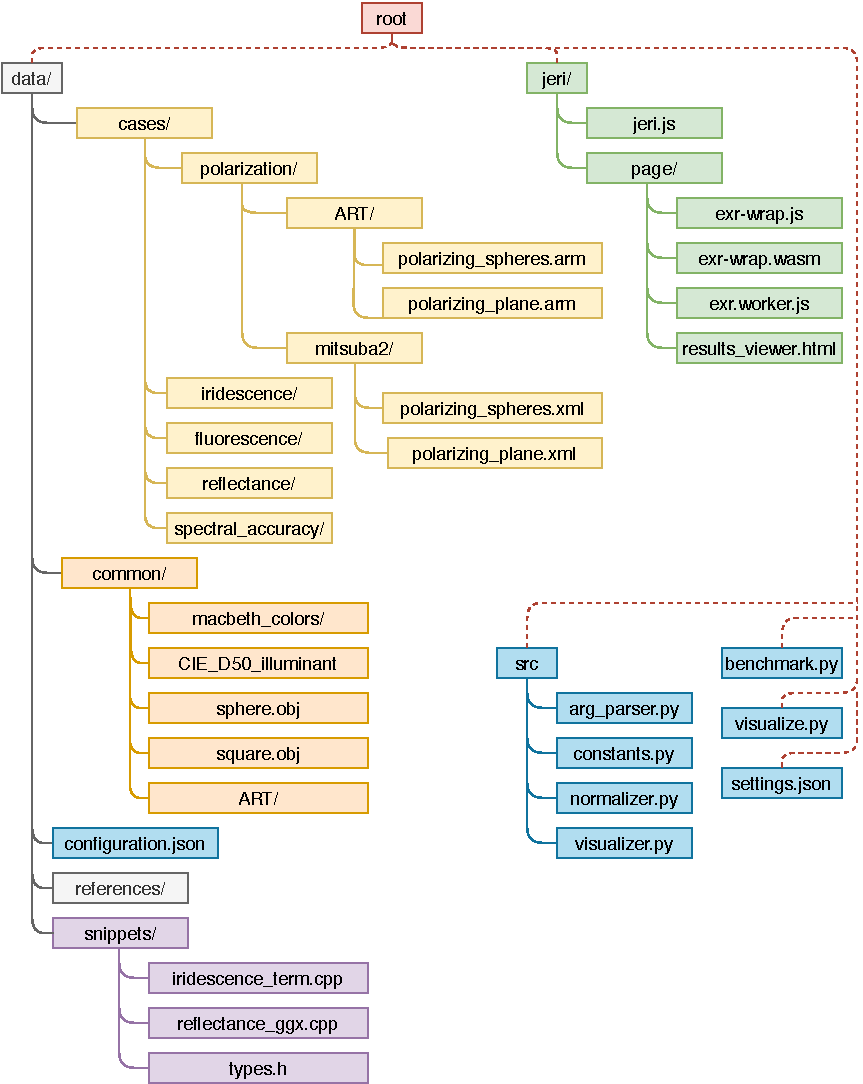
\includegraphics[width=\linewidth]{img/framework.pdf}
	\caption{File organization of the benchmark}
	\label{fig:framework}
\end{figure}

\subsection{Code}

An automated workflow simplifies the evaluation process and ensures that the user is working with the benchmark correctly. The suite consists of several files to accommodate the principle of modularity:

\begin{description}
	\item[{/data/configuration.json}] Contains information about all scenes, test case scenarios, and renderers in a single JSON structure. In case the user wants to add a new scene, a renderer, or a test case scenario, he fills this structure instead of writing new code. A part of the file along with explanatory comments is shown in \autoref{fig:config}.
	\item[/src/arg\_parser.py] Parses the CLI arguments and the \texttt{settings.json} file and fills its variables accordingly.
	\item[/src/configurator.py] Takes the \texttt{/data/configuration.json} file, parses it, and prepares structures for both benchmark script and the results viewing website. In case the \texttt{configuration.json} file is incorrect, it stops the benchmark or simply warns the user to fix it.
	\item[/src/normalizer.py] Normalizes the names of the resulting images after the \\benchmark ends as each renderer might have unique naming conventions. It is used only in corner cases.
	\item[/src/visualizer.py] Runs an HTTP server which is required by JERI (shown in \autoref{sec:jeri}) to upload EXR images and opens the website with the results.
	\item[benchmark.py] A script that is intended to be directly invoked by the user. Runs other helper scripts mentioned above, his purpose is to actually call the rendering executable for each of the scenes found in \texttt{/data/cases/} accordingly to their configurations.
	\item[visualize.py] A script that is intended to be directly invoked by the user. It serves as a wrapper around \texttt{/src/visualizer.py}.
\end{description}

\begin{figure}
	\centering
	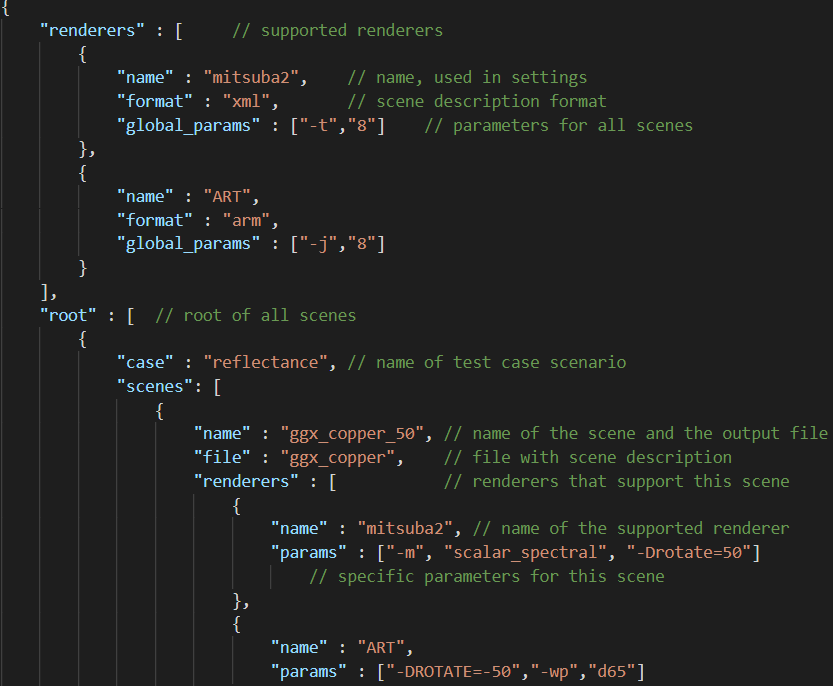
\includegraphics[width=\linewidth]{img/config.png}
	\caption{Part of the configuration file}
	\label{fig:config}
\end{figure}

The choice for Python3 is therefore obvious --- it is a modern, fast, well-known scripting language that is perfectly suitable for our purposes as there is no need for high performance or structurally complicated solutions. Thanks to that, we don't have to force the user to compile the project and the benchmark is immediately ready to use.

\subsection{Cases}

The folder \texttt{/data/cases/} contains the actual scene descriptions along with their configurations. They follow the structure:

\begin{lstlisting}
/data/cases/<case name>/<renderer>/scene
\end{lstlisting}

The benchmark script browses this structure to find each scene specified in \texttt{configuration.json}. The scenes are explained in great detail in \autoref{sec:scenes}.

\subsection{Common data}

The folder \texttt{/data/common/} contains the information and values that are used during the rendering process. The built-in definitions of the geometry or the illumination might be unique for each renderer so it is convenient to have such information in a unified form. The folder contains:

\begin{description}
	\item[macbeth\_colors/] Spectral values for all Macbeth colors --- 24 patch version\footnote{\url{https://xritephoto.com/ph_product_overview.aspx/?id=1192&catid=28}} as defined in ART
	\item[CIE\_D50\_illuminant] Spectral values for CIE D50 illuminant~\cite{cieData} rescaled for Mitsuba2
	\item[rectangle.obj] Square mesh with the length of the side equal to 2
	\item[sphere.obj] Unit sphere mesh
\end{description}

\subsection{Reference images}

The folder \texttt{/data/references/} provides the reference images for each tested scene. Most of these are rendered in Mitsuba2 except for the fluorescent ones which are rendered in ART as the fluorescence is not yet supported by Mitsuba2.

We decided to use the EXR format for the reference images, mostly because we wanted to grant the user as much information as possible for which the typical image formats such as PNG are insufficient. Also, EXR can be considered a standard for the HDR image viewing.

The file \texttt{polarizing\_spheres.exr} is somewhat unique as it contains four different images in four channels. Our visualizer is adjusted to support multi-channel EXRs but in case the user wants to check it manually, he needs a viewer that supports this format.

\subsection{Code snippets}

Some of the evaluated computations at least partially contribute to the material BSDF, hence it is possible to express them in a generalized form that is easily integrable into any conventional renderer. We decided to provide the code snippets written in C++ (stored in the folder \texttt{/data/snippets/}) so that any future user might implement them into his own renderer. The folder contains:

\begin{description}
	\item[iridescence\_term.cpp] Computation of the iridescence term along with the \\helper functions, inspired by the code created by \citet{belcour2017practical}
	\item[reflectance\_ggx.cpp] Contains the methods for sampling, evaluating and masking according to the GGX reflectance definition~\cite{walter2007microfacet}
	\item[types.h] Structures used in the snippets mentioned above 
\end{description}

\subsection{JERI}
\label{sec:jeri}

For the user's convenience, we decided to integrate an EXR visualizer. As it is an addition, we use an existing one instead of creating our own.

\emph{JERI} (Javascript Extended-Range Image) is an EXR viewer written in \\JavaScript and developed by~\citet{jeriWeb}. It is simple to use and to integrate and provides many features over the images such as zoom, change of exposure, and automatic error maps.

We use JERI to display the results of the whole benchmark on a single website. The user may look at the results, the reference images, and even their differences (compared by L1 and SSIM error maps). A screenshot of the results website is shown in \autoref{fig:screenshot}.

Please note that the difference images are supposed to be a helper tool for the user rather than an absolute metric of the correctness. The user is encouraged to use his own difference images or to assess their inconsistencies differently.

\begin{figure}
	\centering
	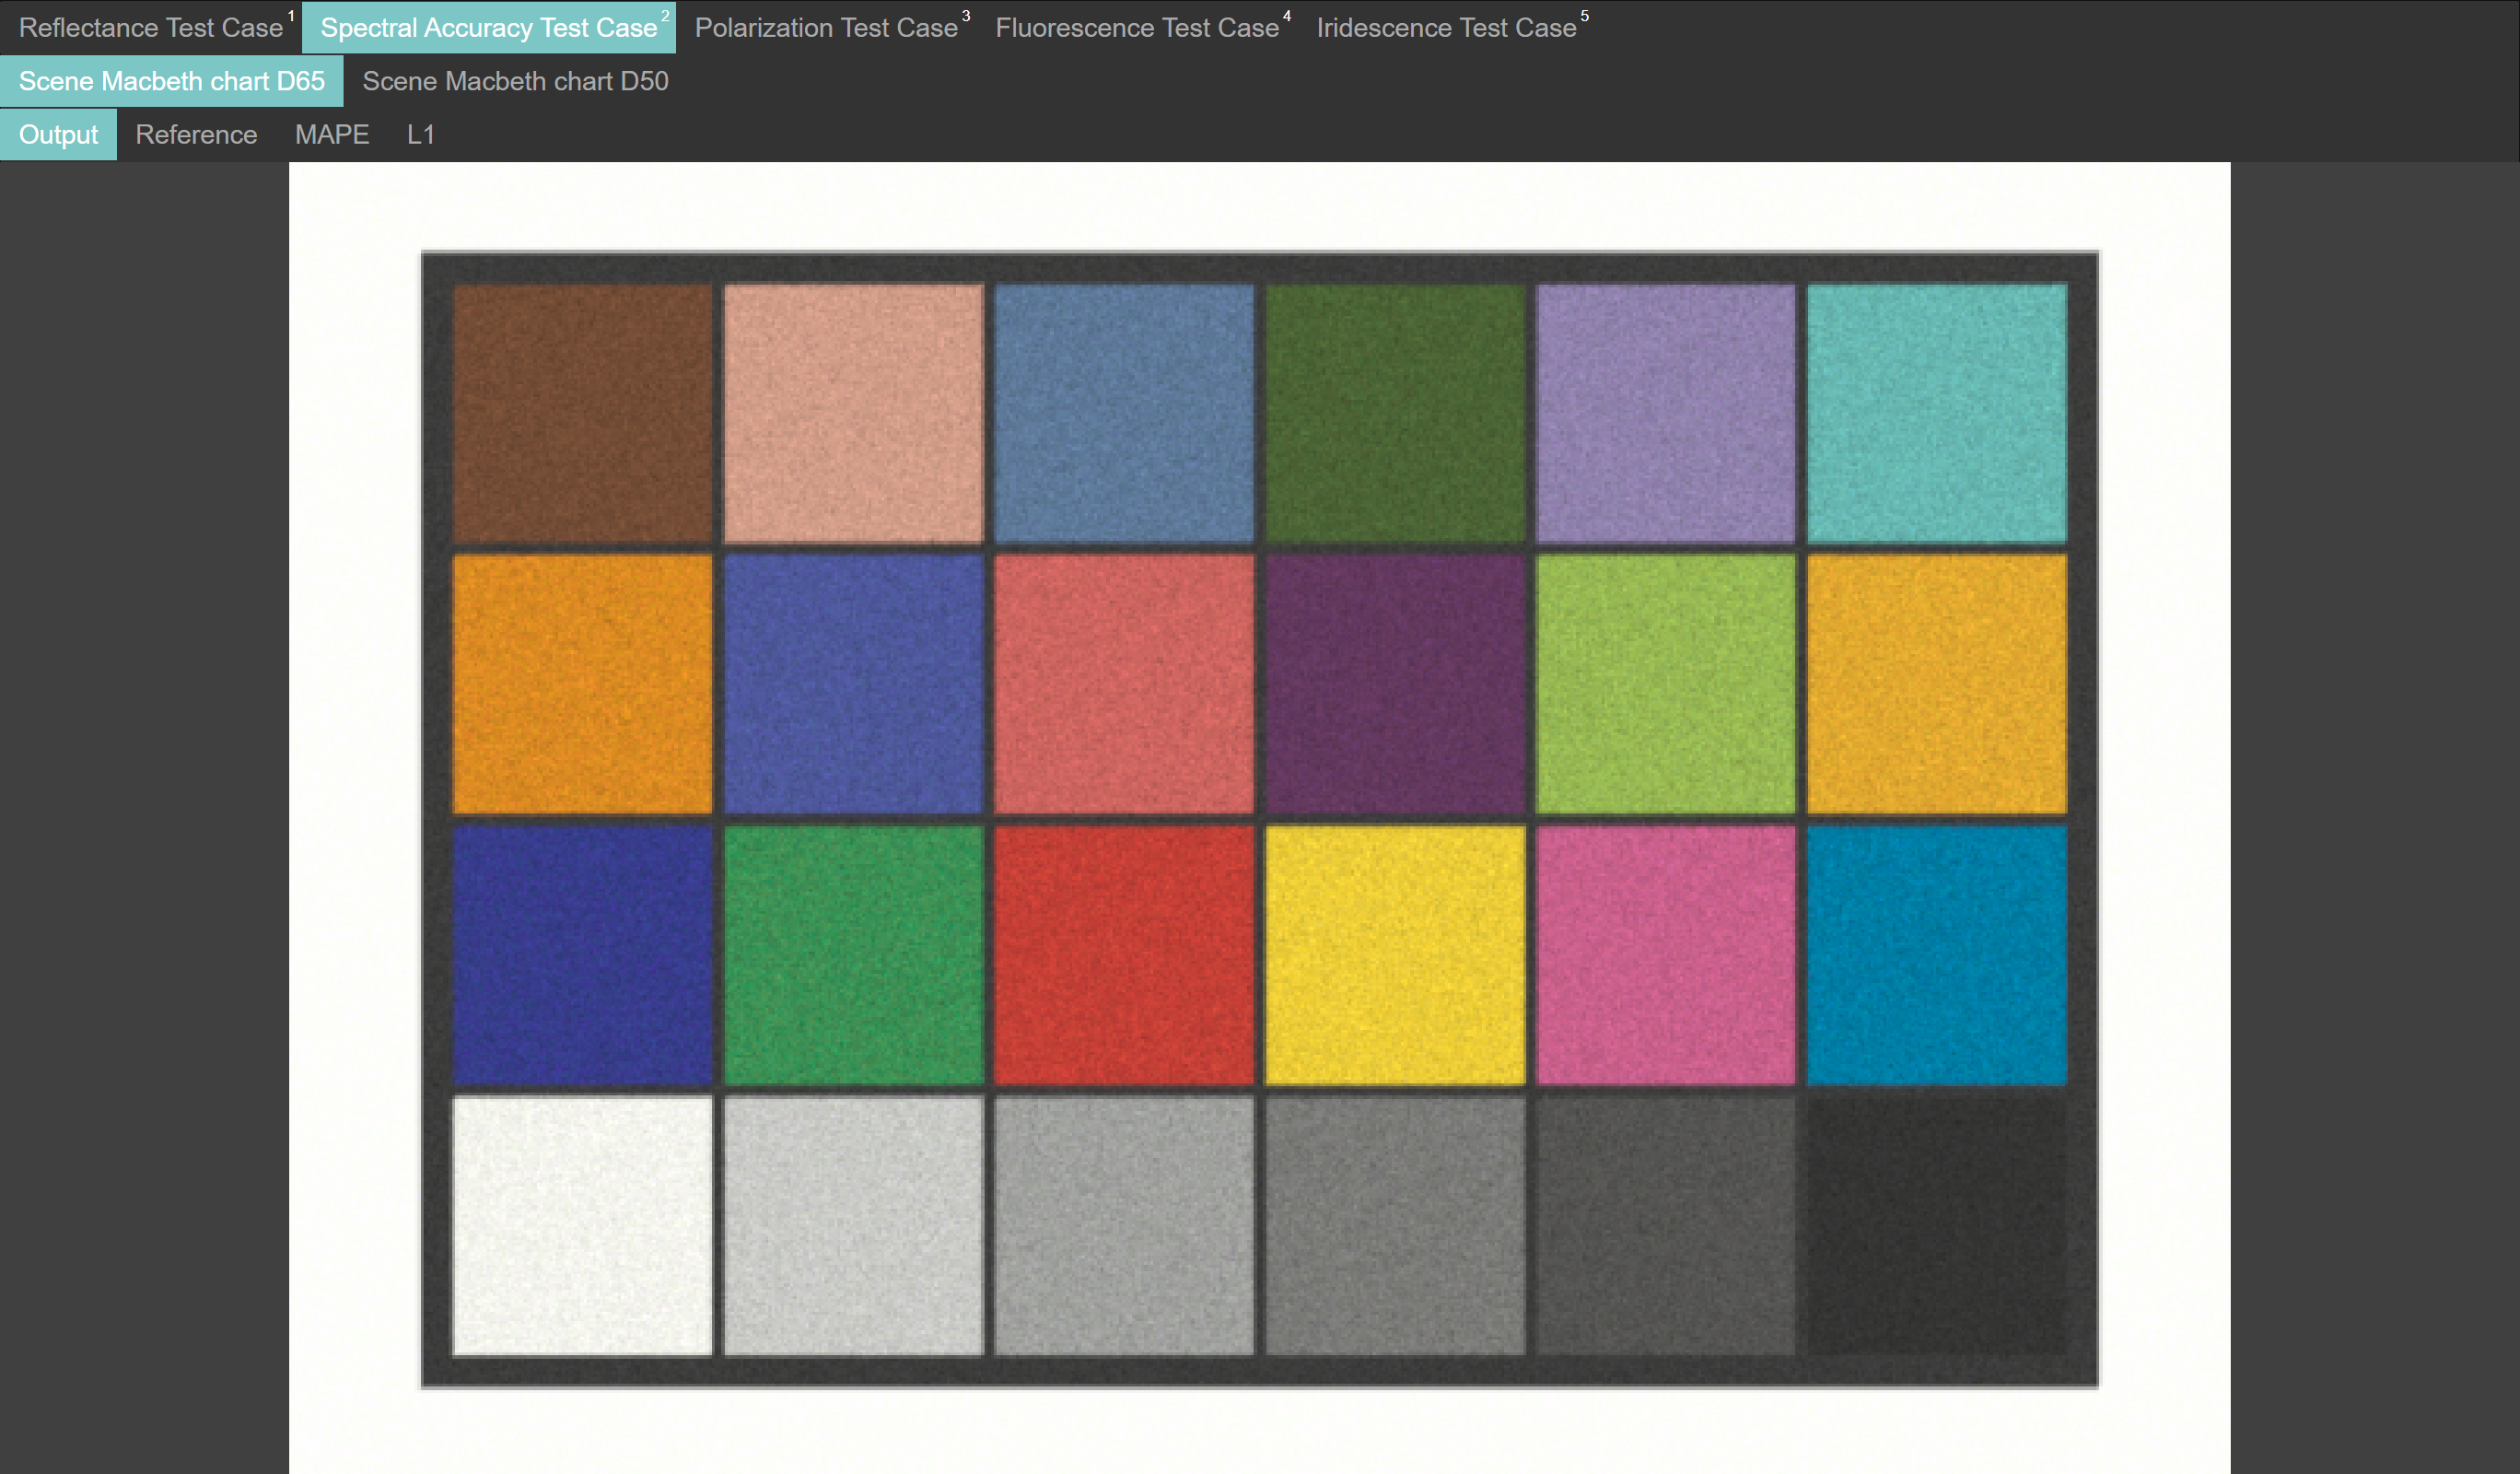
\includegraphics[width=\linewidth]{img/screenshot.png}
	\caption{Results website}
	\label{fig:screenshot}
\end{figure}

\section{Supported Spectral Renderers}

In the current state, the benchmark supports two renderers --- \emph{Mitsuba2} and \emph{ART}. Both are physically-based, research-oriented rendering systems, capable of representing the light in the spectral domain and tracking the polarization states. These features make them suitable candidates for our purposes as we are evaluating the visual correctness of the physically-described appearance phenomena, including spectral accuracy and polarization. The two following sections contain overviews of these renderers.

\subsection{Mitsuba2}

Mitsuba2 has been released only recently (paper was published in November 2019~\cite{nimier2019mitsuba}) as a successor to a well-known, research-oriented renderer Mitsuba 0.6. Rather than an upgrade, Mitsuba2 is a complete overhaul of its predecessor, incorporating the latest trends in programming. It is very well documented by \citet{mitsubaWeb} and \citet{nimier2019mitsuba} and can be downloaded/cloned from \url{https://github.com/mitsuba-renderer/mitsuba2}.

It is written in C++17 and designed to be modular --- it contains a large number of various plugins where each adds new functionality to the Mitsuba2 rendering process, such as:

\begin{description}
	\item[Materials] BSDFs for rough/smooth dielectrics, conductors, plastic, etc.
	\item[Light sources] Uniform, spot, point, area, environment
	\item[Shapes] Imported obj, ply but also built-in geometry such as spheres
	\item[Integrators] Direct illumination, path tracer, stokes integrator, etc.
\end{description}

and many more.

Mitsuba2 is capable of running in several modes --- from RGB CPU rendering to differentiable GPU spectral rendering that tracks polarization. Multiple options can be arbitrarily combined which is illustratively shown in \autoref{fig:mitsuba_variations}. The important part is that the renderer is retargetable which means that the user may specify the rendering mode without recompiling the project. Thanks to the template metaprogramming that C++ offers, Mitsuba2 uses the appropriate internal representation of its data. For example, in RGB rendering, the color is described by an array of 3 floats, each representing red, green, and blue color respectively. In spectral rendering, the array contains 4 floats where each represents the spectral power of a specific wavelength and a stochastic approach is used to sample these wavelengths.

\begin{figure}
	\centering
	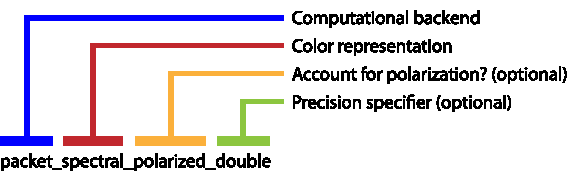
\includegraphics[width=0.8\linewidth]{img/mitsuba_variants.pdf}
	\caption{Different variants of Mitsuba2}
	\label{fig:mitsuba_variations}
\end{figure}

Mitsuba2 also provides an extensive API for Python so that almost all functions may be used from within code. 

Anyone can contribute to the project via a pull request as it is open source.

\subsection{ART}

Advanced Rendering Toolking, or shortly ART, is a physically-based, research-oriented rendering framework that has been developed by the Computer Graphics Group on Charles University in Prague, Faculty of Mathematics and Physics. In the past, there have been important contributions by people at the Institute of Computer Graphics in Vienna. However, as ART is currently at version 2.0.3, most of their work has not been ported from versions 0.x/1.x. ART can be download/cloned from \url{git://cgg.mff.cuni.cz/ART.git} and this section is largely based on its documentation~\cite{artDoc}.

ART is written in Objective-C and therefore compilable on the majority of the modern operating systems. The scenes are written in a custom language that supports procedural modeling of the scene objects, such as loops and conditions. Also, ART generates custom spectral images as the immediate results of the rendering process which contain a lot more information about the wavelengths and the polarization states than standard EXRs. These, however, are not displayable and need to be tonemapped (included in the project) afterward.

On top of the standard features that most conventional renderers offer, such as BSDFs, light sources, camera, path tracing, etc., ART implements several rare, or even unique ones:

\begin{description}
	\item[Spectral rendering] Uses Hero wavelengths spectral sampling
	\item[Fluorescence] Supports fluorescent materials and volumes
	\item[Polarization] Capable of tracking full polarization state of the light
\end{description}

The whole project includes multiple tools such as polarization visualizer or tonemapper which offers several options for adjusting and converting the spectral images.

As ART is an open-source project under GNU v3.0 license, anyone can download and use it.

\section{Methodology}

Before we proceed to the test case scenarios, we should describe the general procedure of adding a new scene to the benchmark. Several steps were followed to design a scene so that it properly examines all essential aspects of a phenomenon while keeping the complexity of the scenes and the amount of them as low as possible:

\begin{description}
	\item[Natural phenomenon] We've studied the behavior of the phenomenon in the nature, i.e. under what circumstances it is perceivable, how does it look like, how to reproduce it, etc. We've also learned the physical models that are behind each of the tested phenomena as their physical properties are properly described.
	\item[Computer graphics research] To test a specific appearance computation, it already has to be developed and embedded inside a rendering system. Therefore, we've looked for the publications and research articles that would show the algorithms used for these computations, the structures and the internal representations of the physical quantities. Furthermore, as we test two open source renderers, we could also study exact implementations that are actually evaluated in the rendering process as these give us all the in-depth information we need.
	\item[Choice of aspects] Based on the research, we've decided what aspects of the phenomena are we going to test. This heavily depends on the specific computation but generally, it is fairly simple to deduce the potential troubles with an algorithm from the scientific publications. They often include measurements and shortcomings of their implementations which greatly simplifies the deductions of the to-be-tested parts. Overall, we take into consideration such computational aspects that are reproducible, easily comprehensible, and most importantly, clearly visible in the final image as the actual assessment is done solely from the reference images. 
	\item[Visualization of aspects] As soon as we've decided on the aspects that are to be exercised, we've designed the scenes that should visualize them. However, we can never fully test all possible combinations as there are, in fact, infinitely many. Therefore, we have aimed to form a minimum number of scenes while maximizing the coverage. This has been quite simple --- many of the phenomena exhibit similar behavior under various circumstances and so they can often be categorized. For example, thicker dielectric layers always exhibit lesser iridescent effects so it does not make sense to try it on different base materials. These categories are then pretty straightforward to describe.
	\item[Manual evaluation] After the scenes are done and they are rendered in the reference renderer, we have manually evaluated each of them based on their physical models and the research papers. This process is supposed to be easy as the scenes were created in a manner that they very clearly display what they were designed for.
\end{description}

\section{Scenes}
\label{sec:scenes}

This section documents all the test case scenarios and the test scenes that we use in our evaluation process. We look into the important objects in the scenes, their meaning and we provide justifications for our decisions. 

Each scene follows the same basic principle --- the geometry is supposed to be as simple as possible. The reference images might not be conventionally eye-pleasing because we are aiming for individual aspects of the specific features that should confirm the correctness of their computations. Also, the number of samples for each scene is generally low, as more samples simply make the picture prettier but do not change (after a certain threshold) the final color.

\subsection{GGX Reflectance}

While we mostly focus on the appearance phenomena caused by the spectral rendering, we include the reflectance of rough surfaces to our benchmark, purely because it is still a largely discussed topic. Specifically, we look into the implementations of the GGX microfacet distribution which, in most cases, is considered to be the the state of the art for rough surfaces. The whole evaluation is based on the publication by \citet{walter2007microfacet}.

This test case scenario consists of five scenes:

The first four scenes are done accordingly to the data measured by \citet{walter2007microfacet}. They are variations of the same scene --- a single rough copper plane under an area light illuminant. Depending on its rotation, various reflected light density is visible throughout the plane, from the strongly illuminated tails at the bottom to the more sparsely distributed direct illumination at the top.

We provide four different rotations --- by 50, 60, 70, and 80 degrees rotated around the x-axis. We believe that such granularity is necessary to be completely sure that none of the viewing/illumination angles breaks the implementation. The copper material provides a visible contrast to the dark background as it is more colorful than other metals such as aluminum or silver. This makes the differences clearly visible even to the naked eye. The roughness is set to 0.2 which can be expressed as considerably rough --- less roughness is meaningless as the differences may not be that visible and more roughness could create an unrealistically rough surface that could be hard to differentiate from a diffuse one. While we could simply put all four planes in one image, we decided to separate them as we wanted to make sure that only one light illuminates one plane at a time from the very spot for each plane. All four scenes are shown in \autoref{fig:ggx_copper}

\begin{figure}[h]
	\begin{tabular}{cc}
		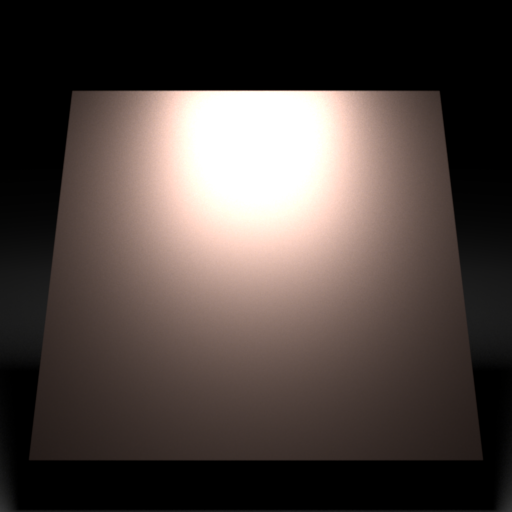
\includegraphics[width=.45\linewidth]{img/ggx_copper_50.png}
		&
		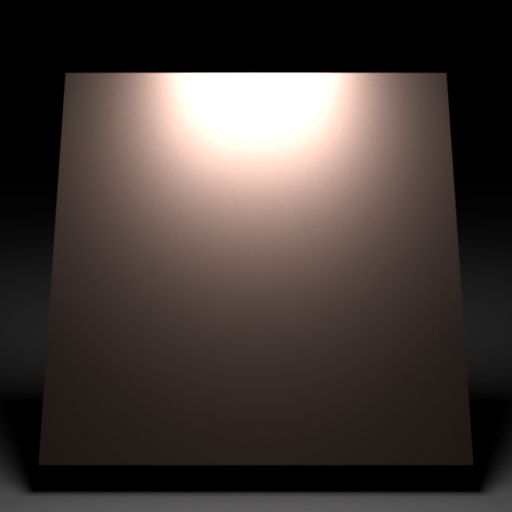
\includegraphics[width=.45\linewidth]{img/ggx_copper_60.png} \\ 
		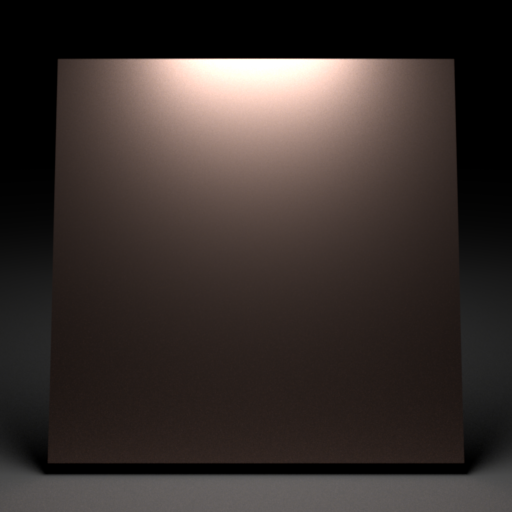
\includegraphics[width=.45\linewidth]{img/ggx_copper_70.png}
		&
		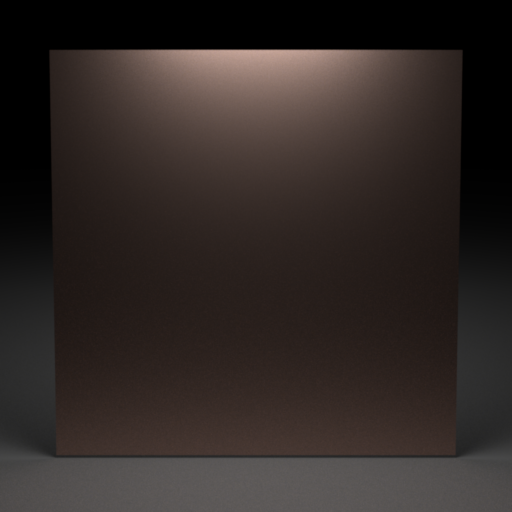
\includegraphics[width=.45\linewidth]{img/ggx_copper_80.png}
	\end{tabular}
	\caption{Four test scenes consisting of a copper plane with GGX distribution}
	\label{fig:ggx_copper}
\end{figure}

While the previous four scenes tested rough conducting surfaces, the fifth scene demonstrates a rough dielectric --- it consists of a single equally rough dielectric sphere under an area light illuminant. We decided to go for a volumetric object instead of the plane for the dielectrics because a dielectric is at least partially transparent and the colors of a plane would predominantly merge with the background. A sphere, however, forms a thick layer in front of the background. Furthermore, testing the very same cases for the dielectrics does not make much sense as we are not testing the material but the microfacet distribution. A sphere also provides various illumination angles where we can potentially spot the inconsistencies between them. This scene converges pretty slowly for such simple geometry because the original GGX implementation needed a quite large number of samples (256 in our case) to render a plausible result. An improvement has been introduced~\cite{heitz2018sampling} that does not change the distribution but greatly decreases variance. As the article~\cite{walter2007microfacet} mostly compares their GGX approach to the Beckmann distribution, we demonstrate our scene rendered for both distributions in \autoref{fig:ggx_glass}

\begin{figure}[h]
	\begin{tabular}{cc}
		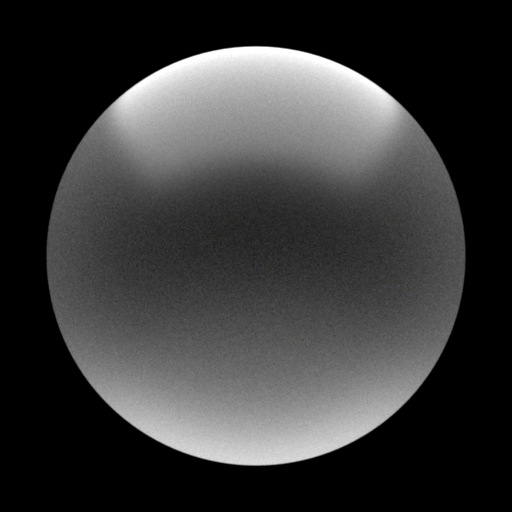
\includegraphics[width=.45\linewidth]{img/ggx_glass.png}
		&
		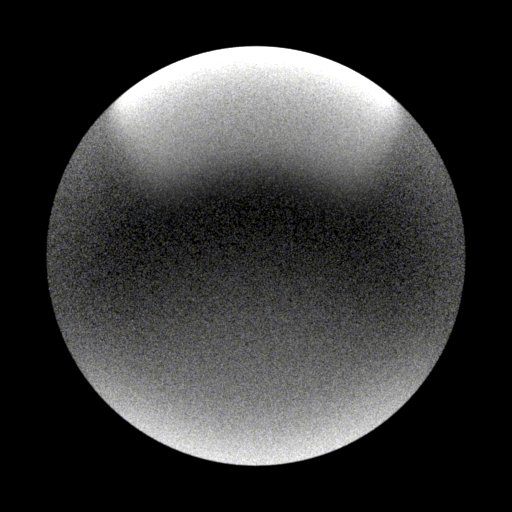
\includegraphics[width=.45\linewidth]{img/beckmann_glass.png}
	\end{tabular}
	\caption{The test scene consisting of a dielectric sphere with GGX distribution (left) compared to its Beckmann equivalent (right)}
	\label{fig:ggx_glass}
\end{figure}

\subsection{Spectral accuracy}

As the direct representation of the spectral colors is not possible on our screens, we need to make sure that the final image contains colors that correspond to the measured data. Distinct renderers may internally represent their color values in a very different manner which might affect the ultimate color that we see.

For these purposes, we use a well-defined set of colors introduced by \citet{mccamy1976color} called \emph{Macbeth chart} or simply \emph{Macbeth colors}. Its basic variant consists of 24 color patches divided in a 4x6 grid, each representing a color that can be normally found in nature --- human skin, flowers, greyscale range, etc. It is primarily used for color calibration therefore it is designed to be stable and invariant under different lighting conditions.

We introduce two scenes that evaluate the correctness of the spectral colors --- both contain a Macbeth chart illuminated by two different standard CIE illuminants, D50 and D65~\cite{cieIlluminants}. As both illuminants and Macbeth colors have exact definitions, they are easily integrated into any renderer that supports spectral color representation. Another advantage is that we know their corresponding RGB values so the results can be easily checked against them.

We assume that the white point of the renderer is CIE D65 (whitepoint of sRGB) for both scenes. Thus, the scene illuminated by the D50 illuminant should have an orange-ish overlay and the scene illuminated by the D65 illuminant should have a completely white background.

Both scenes are shown in \autoref{fig:macbeth}. Once the renderer passes this test, we can assume that the representation of the spectral colors is indeed correct. Even though this may seem trivial, testing multiple different materials, colors or even illuminants is simply a variation of our tests with the only difference that we need to evaluate the correctness manually as we do not have the color definitions beforehand.

\begin{figure}[h]
	\begin{tabular}{cc}
		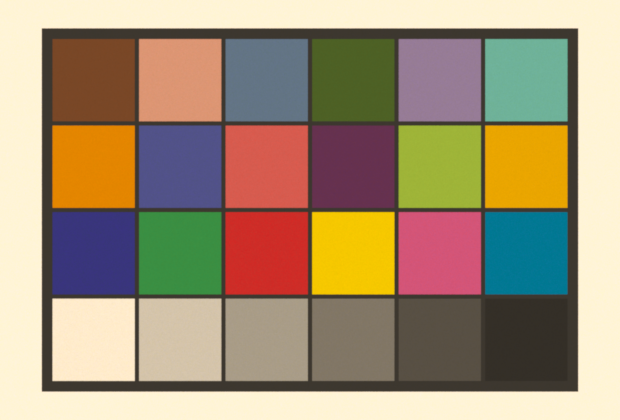
\includegraphics[width=.45\linewidth]{img/macbeth_chart_D50.png}
		&
		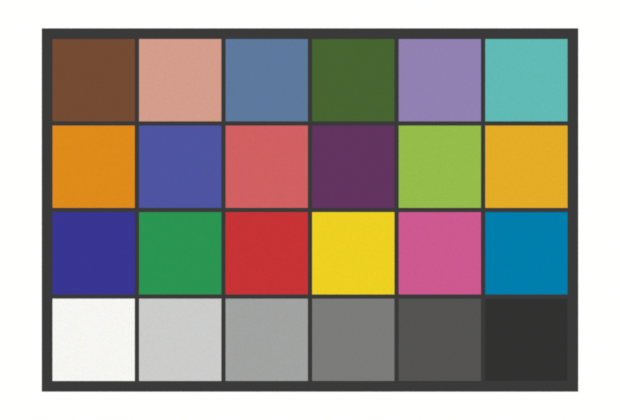
\includegraphics[width=.45\linewidth]{img/macbeth_chart_D65.png}
	\end{tabular}
	\caption{The test scenes containing a Macbeth chart under CIE D50 illuminant (left) and CIE D65 illuminant (right)}
	\label{fig:macbeth}
\end{figure}

\subsection{Polarization}

The polarization cannot be described by a BSDF as GGX or iridescence. It requires full tracking of the polarization states during the rendering process and ideally a tool that would display these states. Fortunately for us, both ART and Mitsuba2 provide a way to display the results of the Stokes vector as well as polarization filters that are ideal for these kinds of experiments.

The first two scenes use Brewster's angle (explained in \autoref{sec:polarization}) --- they contain a perfectly reflective dielectric plane (IOR of glass = 1.52) that is illuminated by a single area light under Brewster's angle. By the definition, the light reflected from the plane is perfectly p-polarized. The difference between the two scenes is in the linear polarizer situated in front of the camera --- in case the transmission axis is horizontally oriented (parallel to the reflected light), the reflection of the light source is clearly visible without any attenuation. However, if the transmission axis is vertically oriented (perpendicular to the reflected light), there is no reflection of the light source on the plane as the polarizer won't simply let it through. Both scenes are shown in \autoref{fig:polar_planes}.

\begin{figure}[h]
	\begin{tabular}{cc}
		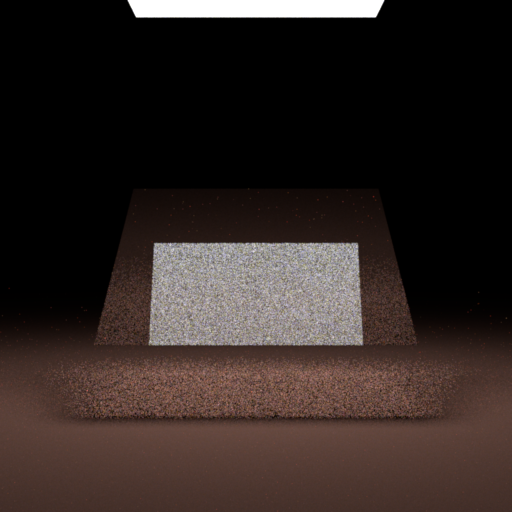
\includegraphics[width=.45\linewidth]{img/polarizing_plane_90.png}
		&
		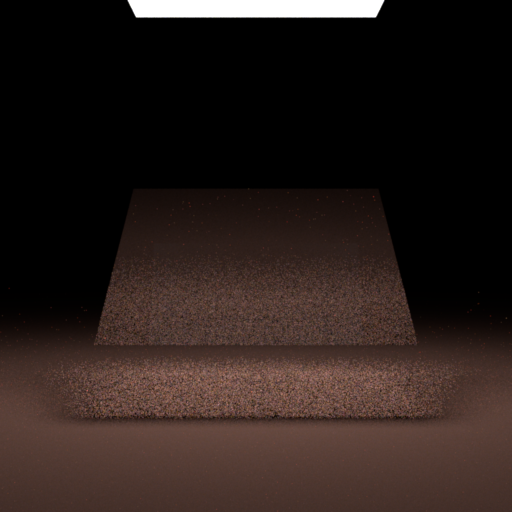
\includegraphics[width=.45\linewidth]{img/polarizing_plane_0.png}
	\end{tabular}
	\caption{The test scenes with a visible polarized (left) and without a visible polarized light (right)}
	\label{fig:polar_planes}
\end{figure}

The third scene is a lot more specific as it heavily depends on the renderer to be capable of representing the polarization via Stokes vectors and visualizing their components. This scene contains two smaller dielectric spheres that are in front of a larger smooth conducting sphere illuminated by a constant daylight. Thanks to the constant surrounding light, lots of transmissions and reflections are happening from the dielectric spheres which consequently polarizes the light.

Note that to ensure physical plausibility, the scenes are monochrome at 550nm wavelength. In ART, it is possible to extract the single wavelength information image from its custom spectral image format. In Mitsuba2, we used a workaround by specifying only the 550nm values of all colors inside the scene (light and floor) and by running the rendering process in the monochrome mode.

Both Mitsuba2 and ART output their results as four distinct images, each representing a different element of the Stokes vector (the complication with the compatibility of the outputs and its solution is explained in \autoref{sec:multichannel_jeri}). All four images are shown in \autoref{fig:polar_spheres}. Pay attention to the fourth image, which demonstrates that the circular polarization is also happening with the reflections of the dielectric spheres on the conducting one.

\begin{figure}[h]
	\begin{tabular}{cc}
		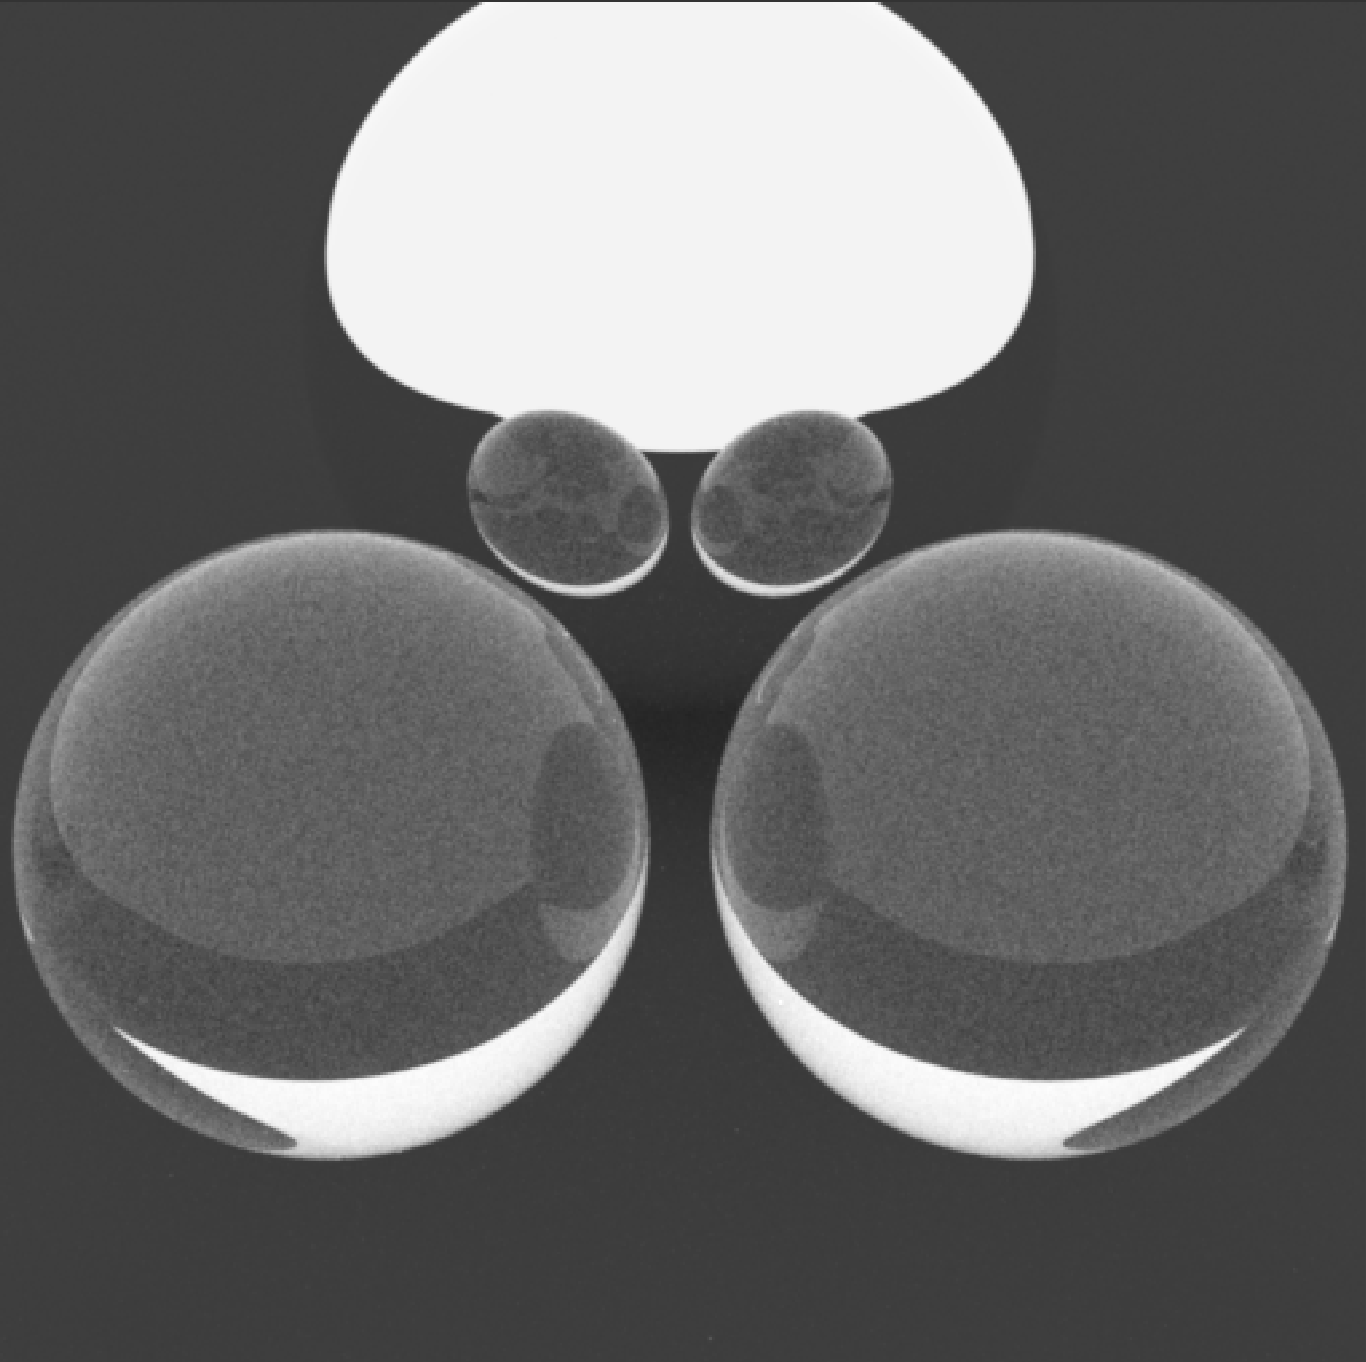
\includegraphics[width=.45\linewidth]{img/polarizing_spheres.s0.png}
		&
		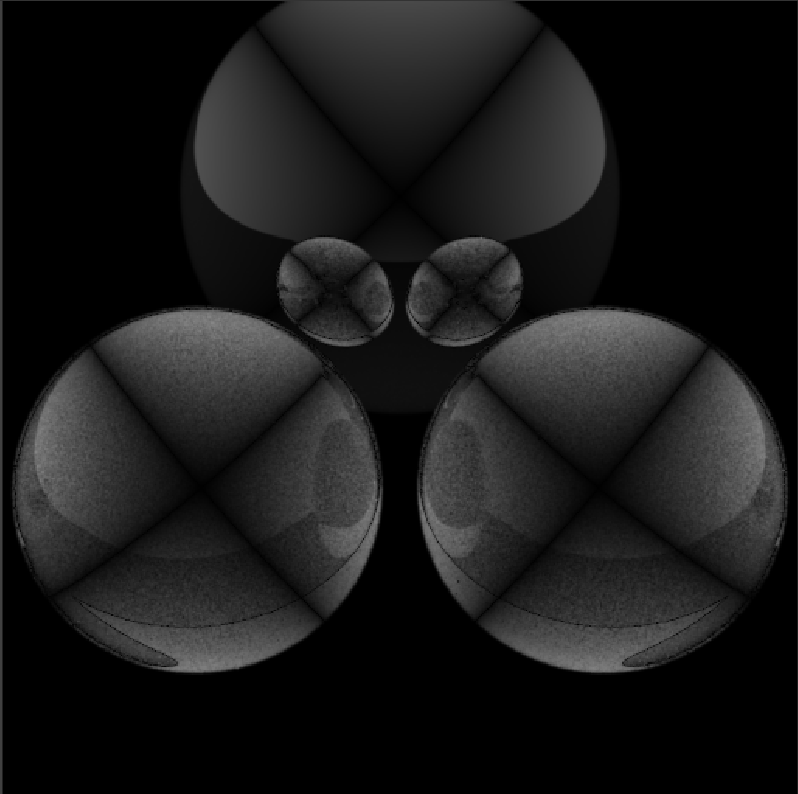
\includegraphics[width=.45\linewidth]{img/polarizing_spheres.s1.png} \\
		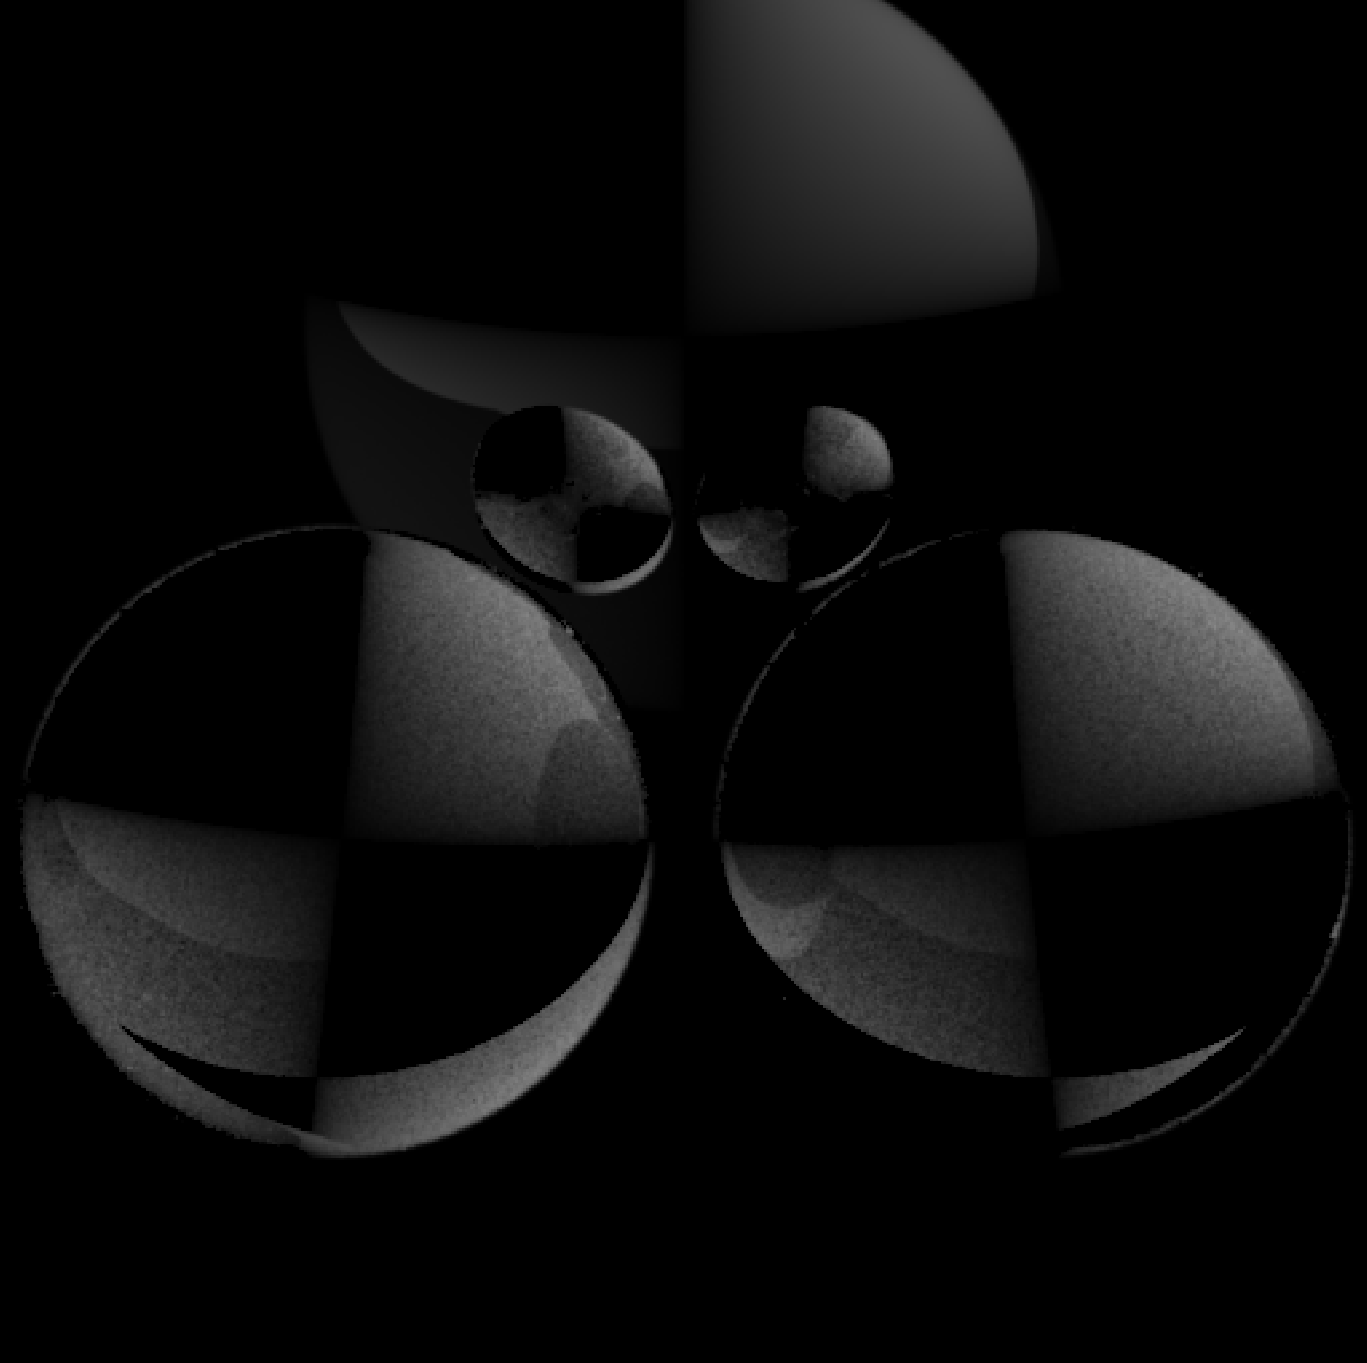
\includegraphics[width=.45\linewidth]{img/polarizing_spheres.s2.png}
		&
		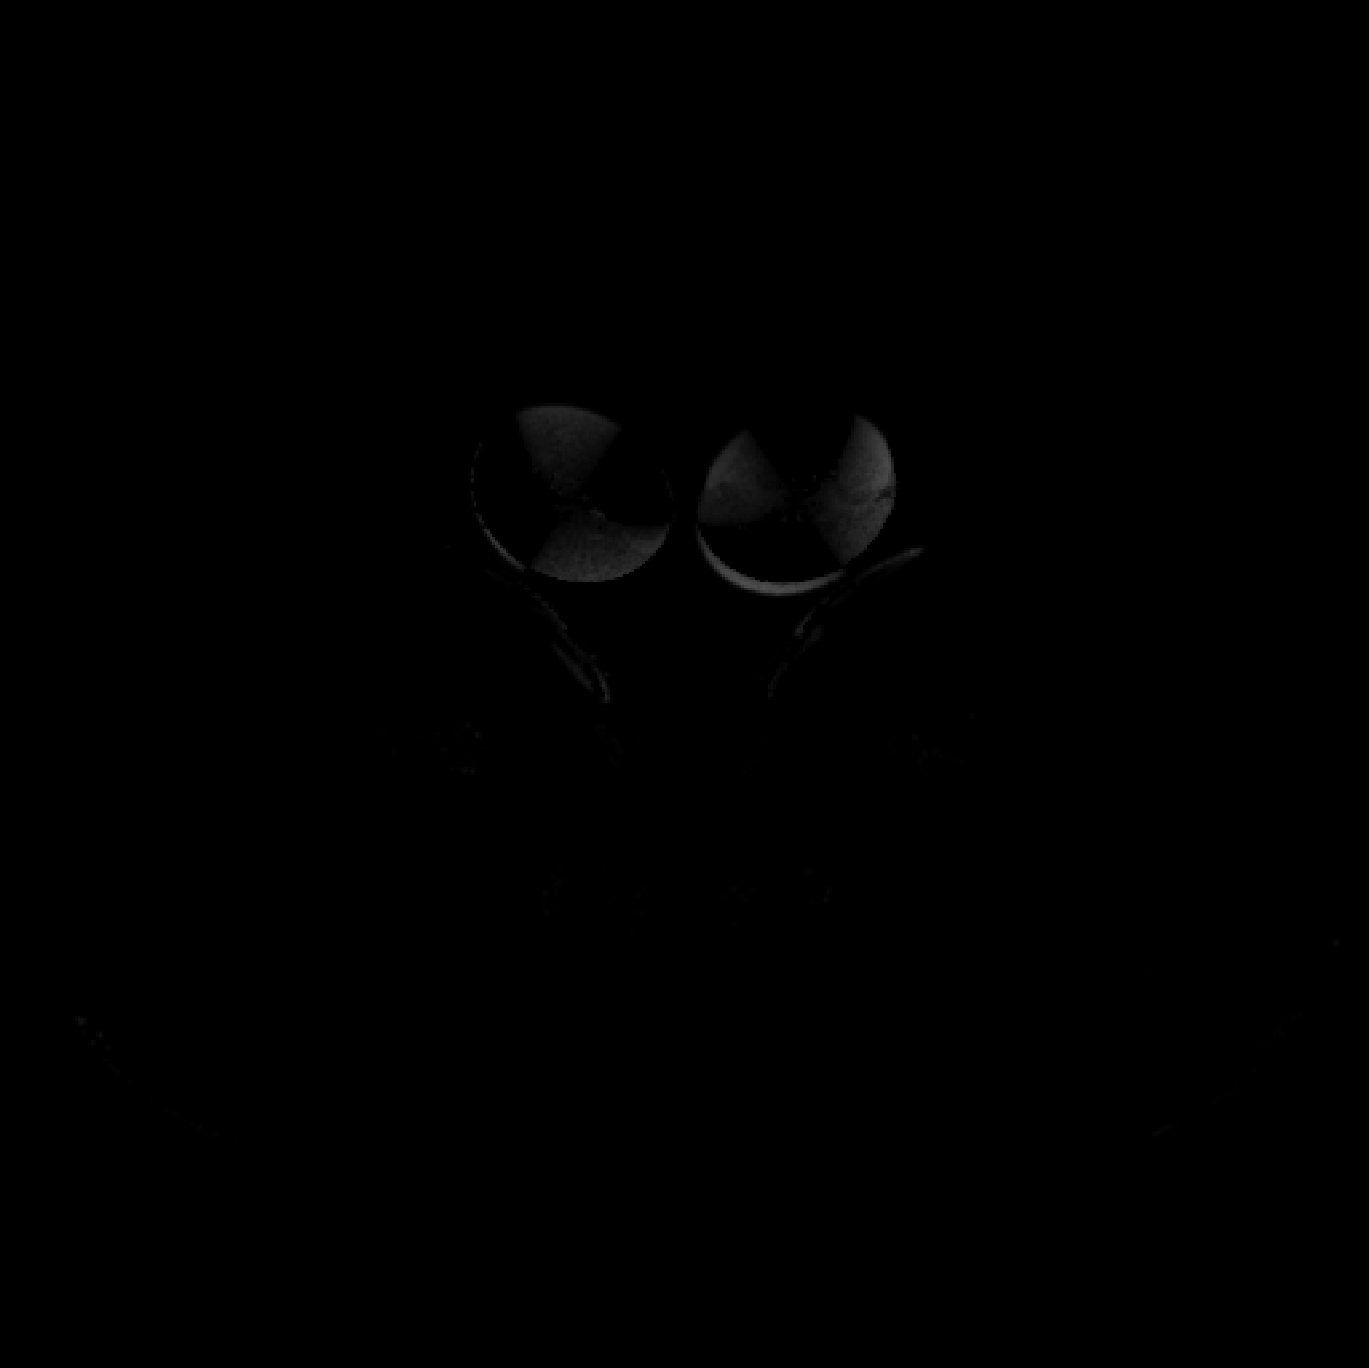
\includegraphics[width=.45\linewidth]{img/polarizing_spheres.s3.png}
	\end{tabular}
	\caption{The four Stokes vector outputs of a test scene containing polarizing spheres}
	\label{fig:polar_spheres}
\end{figure}

\subsection{Fluorescence}

Fluorescence is one of the four phenomena that are possible thanks to the spectral rendering. As it can be perceived only under rare circumstances, its implementation has been purposely avoided in the vast majority of the renderers. However, as physical realism begins to be a must-have in the commercial world, the interest in its integration grows.

We provide four different test scenes that exercise the fluorescent materials and illuminants and their properties accordingly to their natural behavior. In this case, only ART scenes are provided as Mitsuba2 does not support the feature. 

The test scenes take inspiration from the implementation of fluorescence by \citet{mojzik2018handling}. They all consist of a single yellow-based sphere whereas its properties are essentially various combinations of the absorption spectrum, emission spectrum, and the surrounding constant illumination.

\begin{description}
	\item[D50, 370nm absorption, 650nm emission~\ref{fig:fluorescence_d50_red}] The sphere absorbs 370nm \\wavelengths and re-emits 650nm while it is placed under the CIE D50 horizon light illuminant. As you can see, the sphere displays a yellow to orange color which is a combination of the yellow base and the emitting red color --- 650nm wavelength is perceived as red. The reason that the sphere is not completely red is due to the lower spectral power of the D50 illuminant around 370 nanometers wavelengths.
	\begin{figure}[H]
		\centering
		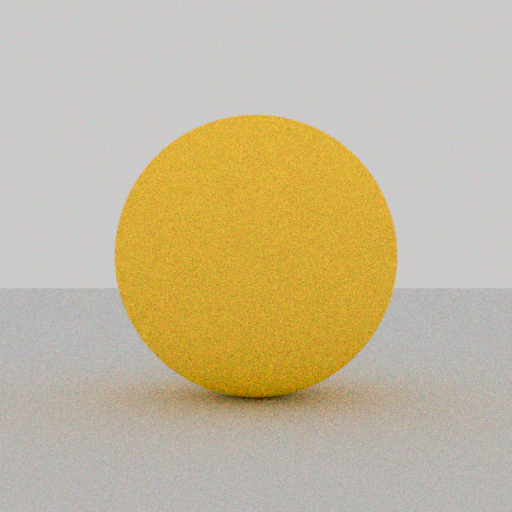
\includegraphics[width=.6\linewidth]{img/fluorescent_sphere_D50_red.png}
		\caption{}
		\label{fig:fluorescence_d50_red}
	\end{figure}
	\item[450nm illuminant, 450nm absorption, 650 emission~\ref{fig:fluorescent_sphere_mono_red}] The sphere absorbs 450nm wavelengths and re-emits 650nm while it is placed under a monochrome light, emitting 450nm wavelengths only (perceived as blue). Intuitively, as the absorption spectrum and the illuminating spectrum collide, the sphere should emit a bright red color.
	\begin{figure}[H]
		\centering
		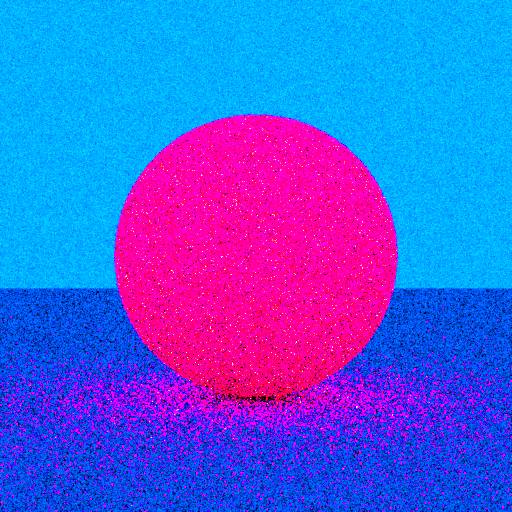
\includegraphics[width=.6\linewidth]{img/fluorescent_sphere_mono_red.png}
		\caption{}
		\label{fig:fluorescent_sphere_mono_red}
	\end{figure}
	\item[450nm illuminant, 370nm absorption, 650 emission~\ref{fig:fluorescent_sphere_mono_invisible}] The sphere absorbs 370nm wavelengths and re-emits 650nm while it is placed under a monochrome light, emitting 450nm wavelengths only (perceived as blue). In this case, the two spectral domains do not collide at all. Therefore, the sphere appears to be black due to the missing emission and its opaque surface as there is simply no light to absorb and consequently nothing to emit. Note that a dielectric would be completely transparent but we do not test this case as it does not concern fluorescence directly but rather the material itself.
	\begin{figure}[H]
		\centering
		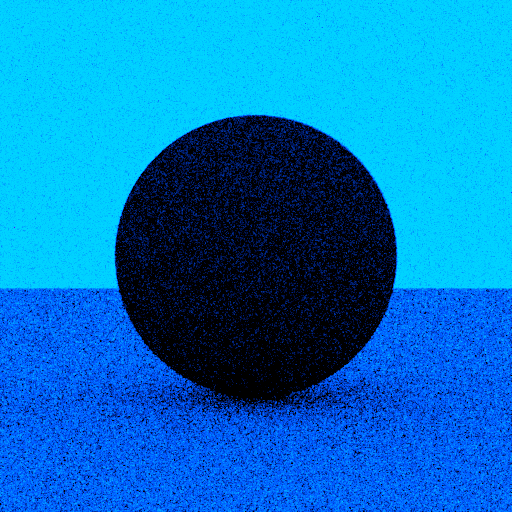
\includegraphics[width=.6\linewidth]{img/fluorescent_sphere_mono_invisible.png}
		\caption{}
		\label{fig:fluorescent_sphere_mono_invisible}
	\end{figure}
\end{description}

Many more combinations testing different emitting/absorbing spectral domains and illuminants are possible, however, we believe that they would only be variations of the four test case scenarios mentioned above --- normal light with a fluorescent sphere, monochrome light with a sphere absorbing different wavelengths and monochrome light with a compatible sphere. We do not test fluorescent illuminants on purpose as these, from the technical point of view, have nothing do the with fluorescent effects but they are using fluorescent materials inside them.

\subsection{Iridescence}

The evaluation of the iridescence showed some complications as neither Mitsuba2 nor ART natively support the iridescent effects. The only implementation we found was for Mitsuba version 0.6 introduced by \citet{belcour2017practical}.

We've reimplemented the plugin to Mitsuba2 and used the Mitsuba 0.6 implementation as a reference. The results of the tested scenes were identical so we can safely consider the Mitsuba2 images as the ground truth.

The implementation simulates the iridescence caused by the light interference in a very thin dielectric film on top of a rough conducting base. Three parameters can be set for this iridescent BSDF --- the IOR of the exterior, the IOR of the film and the height of the film. Unfortunately, the final colors of the iridescent effects change rapidly with every slight variation of the parameters of both the conducting base and the dielectric film. Despite that, there are some consistent changes with the gradual increase of the film height and the film IOR which we are exposing in our test scenes. 

Each scene consists of four spheres surrounded by constant daylight to see the colors as brightly as possible. These spheres have a very low roughness coefficient ($\alpha=0.1$) so that the rough surface does not distort the effect.

\begin{description}
	\item[Film height~\ref{fig:irid_height}] As we've explained in \autoref{sec:irid}, the increasing thickness of the film reduces the visibility of the iridescent effect as there is less light interference. All spheres in this scene have identical base and film IOR --- $\eta_{base}=1.9, \kappa_{base}=1.5, \eta_{film}=1.33$. The first two spheres with the film height equal to 300nm and 550nm are displaying equally visible iridescent effects. The difference is, of course, in their colors as the light interference is largely varying. The film height of the third sphere is quite high, 1500nm, which clearly diminishes the iridescent effect, dominantly displaying its base color. For the reference, the fourth sphere has no film layer on top of it, displaying only the base.
	\begin{figure}[H]
		\centering
		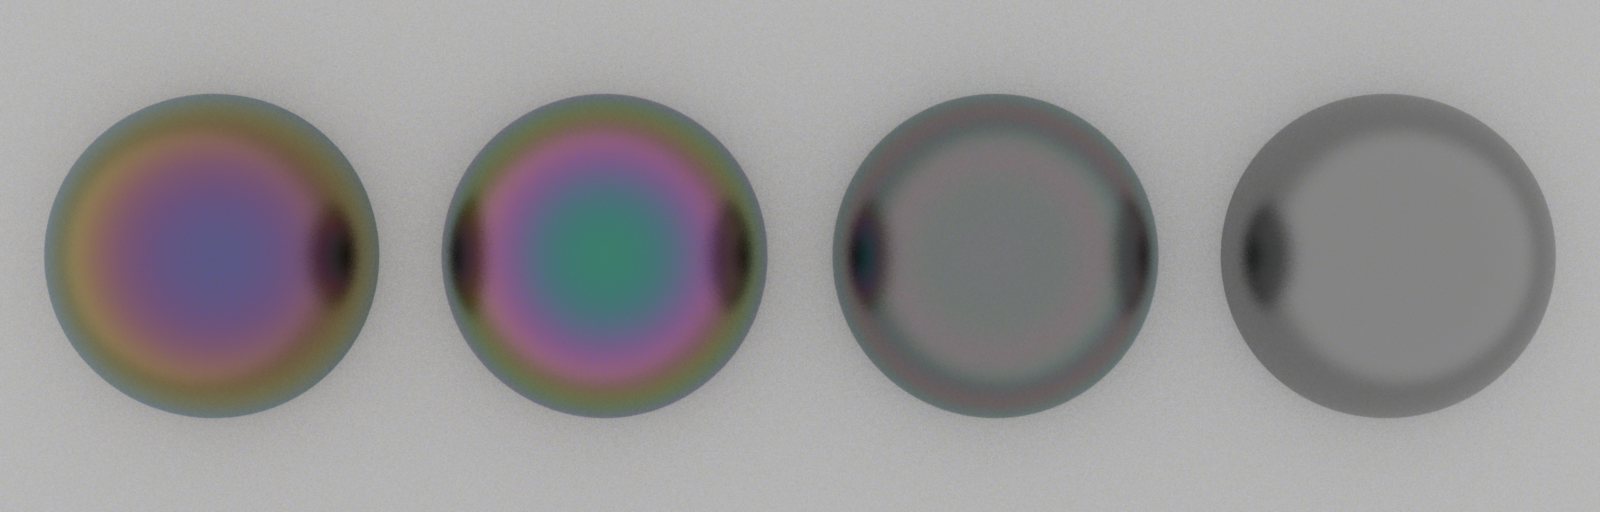
\includegraphics[width=.9\linewidth]{img/iridescent_spheres_height.png}
		\caption{}
		\label{fig:irid_height}
	\end{figure}
	\item[Film IOR~\ref{fig:irid_ior}] Another apparent change happens upon the adjustments to the film IOR. With the decreasing IOR of the film, more color fringes can be spotted on the sphere. From the definition of IOR (essentially, how much faster light travels in the vacuum than in the current medium), we can deduce that the faster the light travels through the medium, the interferences happen at a higher rate and therefore we can see more colors. The spheres in this scene have identical base and the film height --- $\eta_{base}=1.9, \kappa_{base}=1.5, film\_height=550nm$. The film IORs $\eta_{film}$ are equal to 1.2, 1.5, 1.8 and 2.8, where each consecutive sphere displays one less color fringe that the previous one (from 5 to 2). Please note that the counted amount of the color fringes is not an absolute measure but rather a rough approximation done by naked eye --- there are a lot more colors in-between gradiently transitioning between the fringes and the user may have counted them differently.
	\begin{figure}[H]
		\centering
		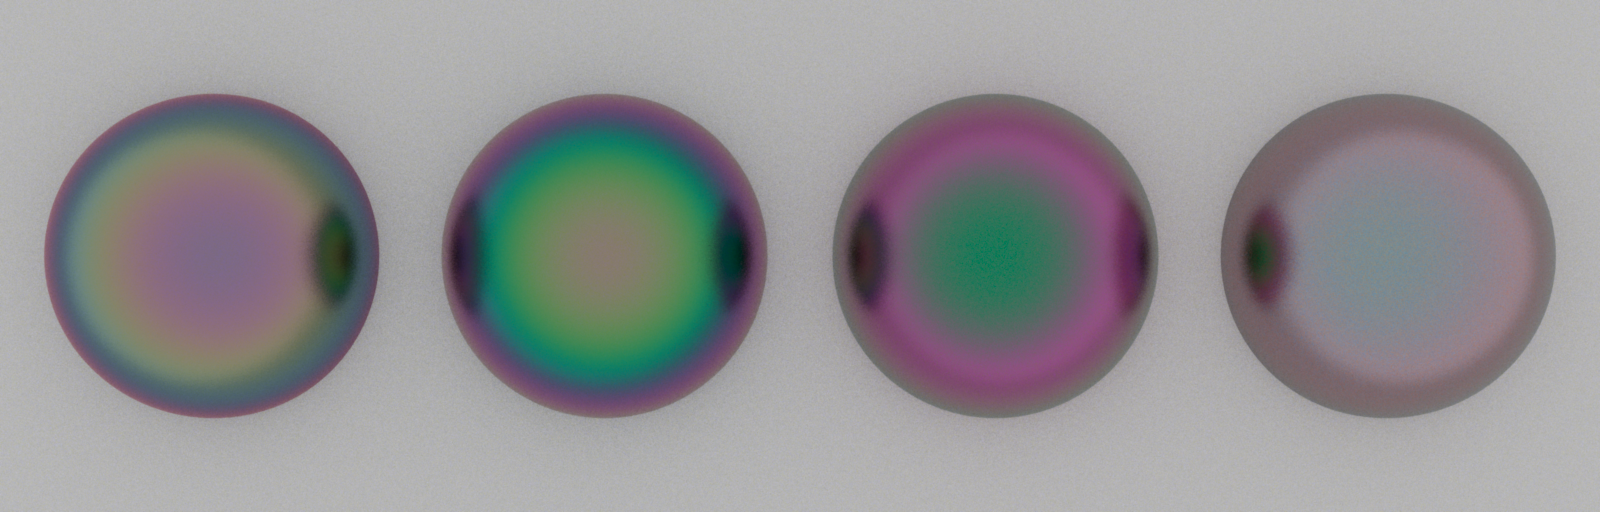
\includegraphics[width=.9\linewidth]{img/iridescent_spheres_film.png}
		\caption{}
		\label{fig:irid_ior}
	\end{figure}
	\item[Materials~\ref{fig:irid_mat}] The last scene demonstrates a direct comparison between two well-defined materials (their properties $\eta_{base}$ and $\kappa_{base}$ provided by Mitsuba) --- copper and mercury --- and their iridescent equivalents with $\eta_{film}=1.33,film_{height}=550nm$. Both materials emit the same iridescent effect simply put on a  different color base.
	\begin{figure}[H]
		\centering
		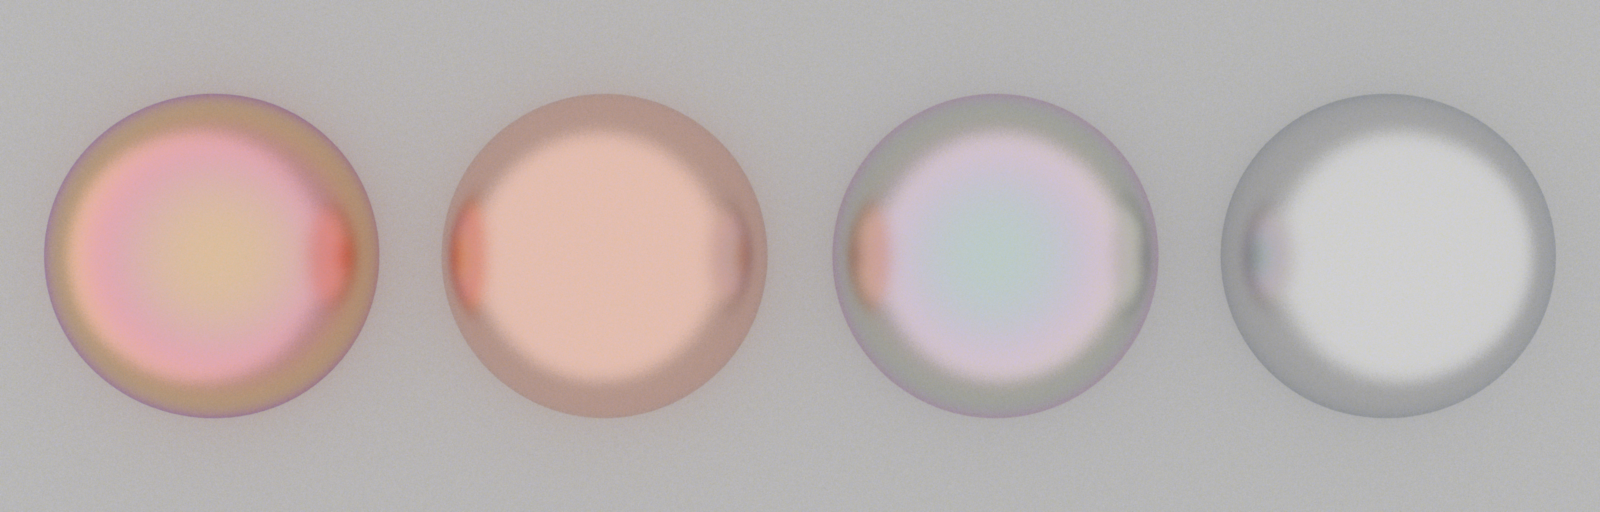
\includegraphics[width=.9\linewidth]{img/iridescent_spheres_materials.png}
		\caption{}
		\label{fig:irid_mat}
	\end{figure}
\end{description}

Due to the custom implementation of this plugin for Mitsuba2, we do not evaluate ART is it does not support iridescence at all.

\subsection{Dispersion}

Unfortunately, we do not provide any test scenes for dispersion. Mitsuba2 simply does not support the feature which is also explicitly stated in their documentation. ART supports dispersion but we've encountered some issues with the darker colors of the dispersive materials and so we cannot declare the images displaying dispersion generated by ART as the ground truth.

\section{Use cases}

In the following sections, we demonstrate the basic uses cases of our testing suite.

\subsection{Use case Regress test}

A user who recently changed an essential but not directly tested part of the renderer (e.g. sampling strategy) wishes to confirm that he did not break any other functionality. He downloads our benchmark and inserts his latest executable. Then, he runs all test case scenarios and compares the results with the reference images. Refer to the user guide for more information about the usage of the benchmark~\ref{user_guide}.
 
\subsection{Use case New feature}
\label{sec:frodo}
A user wishes to implement one of the tested features to a rendering system that is not yet evaluated for that specific scenario but generally supported by the benchmark (e.g. GGX microfacet distribution to ART). He wishes to check the correctness of its implementation so he follows these steps:

\begin{enumerate}
	\item If provided, find the code snippets that are attached to the benchmark suite and integrate them to the renderer.
	\item Duplicate the scenes prepared for other renderers that test the feature and store them in a new \texttt{/data/cases/feature/renderer/} folder. This step should be straightforward as the objects inside the scenes are fairly basic and commented.
	\item For each affected scene, add a JSON snippet to \texttt{configuration.json} file containing the newly supported renderer's name and its parameters (look at \autoref{fig:config}).
	\item Insert the latest executable to the benchmark and run it.
\end{enumerate}

The benchmark automatically detects the new configuration. Either from the reference images or the difference images, the user may now run the evaluation to assess the accuracy of the newly implemented feature.

\subsection{Use case New scenario}

A user who wishes to add a completely new test case scenario must follow these few steps:

\begin{enumerate}
	\item Add a new folder to the benchmark suite \texttt{/data/cases/new\_scenario/}
	\item Add JSON snippet for the new scenario to the \texttt{configuration.json} file
\end{enumerate}

From now on, the benchmark automatically evaluates this feature as well. If the user wants to provide the reference images, these need to be stored in the \texttt{/data/references} folder.

\subsection{Use case Improved feature}

A user who improved a specific feature and wishes to confirm his assumptions may use the benchmark in a standard way.

The scene descriptions may be considered as templates used to create the reference images. In case some structural changes were done inside the renderer, such as variable names, the scenes can be easily adjusted to comply with the new renderer.

If he finds out that the results indeed improved, he may replace the existing scene descriptions, as well as the reference images, for the better, adjusted ones.

\subsection{Use case New renderer}

A user who wishes to add support for a new renderer into the benchmark suite must follow these steps::

\begin{enumerate}
	\item Create a new folder with the name of the renderer for each test case scenario in the \texttt{/data/cases/}
	\item Rewrite the template scenes from other renderers to his own scene format
	\item Store these scenes in the newly created folders accordingly
	\item Add the renderer's name to the array containing all supported renderers at the beginning of the  \texttt{configuration.json} file
	\item For each scene, add a JSON snippet to the \texttt{configuration.json} file containing the newly supported renderer's name and its parameters.
	\item Insert the latest executable to the benchmark and run it.
\end{enumerate}

\section{Open source contributions}

During our work on the benchmark, we have done several noteworthy contributions to three open-source projects. Note that these extensions can be considered as byproducts and not the main aim of this thesis --- therefore, they are not yet in a state that can be used for a pull request as this process requires a significant amount of time.

\subsection{GGX for ART}

The use case described in \autoref{sec:frodo} happened to us. We've decided to add the GGX distribution to the ART renderer and, coincidentally, it correlated with the mentioned scenario. We had the scenes and the reference images prepared for Mitsuba2, we simply replicated them for ART and implemented the GGX. Then, as mentioned in the use case, we iterated the benchmark and the adjustments in the code over and over until the results were satisfactory.

The implementation can be found in the attachments of the thesis in \autoref{sec:ggx_art}.

\subsection{Iridescence for Mitsuba2}

Mitsuba does not have native support for the iridescence but an external plugin has been developed to simulate the iridescent effects of a thin film dielectric layer on top of a rough conductor base. Unfortunately, it was created for Mitsuba version 0.6 and, as Mitsuba2 is fairly new, there has not been an effort to rework the plugin, thus we took the initiative and re-implemented it.

Along with the publication done by \citet{belcour2017practical}, they released a supplementary plugin for Mitsuba 0.6 to demonstrate their results.

There were some major changes to the spectral sampling strategy and the overall object structure done in Mitsuba2 that had to be adapted in the new, re-implemented version of the plugin.

The correctness of the rework has been confirmed in similarly to the normal evaluation workflow. We prepared the test case scenario scenes for the iridescence, rendered them for both Mitsuba2 and Mitsuba 0.6, and considered the latter version to be the ground truth. The implementation can be found on \url{https://github.com/marcel1hruska/mitsuba2} or in the attachments of this thesis~\ref{sec:mitsuba2_irid}.

\subsection{Multi-channel EXR support for JERI}
\label{sec:multichannel_jeri}

While designing the polarization test scenes, we've encountered a compatibility issue between the Stokes vector output format of Mitsuba2 and ART. While ART stores the Stokes vector values into distinct EXR images, Mitsuba2 creates a single multi-channel EXR where each channel contains the Stokes vector information. As you can imagine, such a visualization of the rendering results requires a custom solution.

First of all, we've added general support for multi-channel EXR images to the JERI framework as there is currently no way to visualize them. It works as follows:

\begin{enumerate}
	\item If the EXR image contains multiple channels, store them in a structure called \texttt{otherChannels} which maps the channel name with its contents.
	\item The user may specify the channel to display similarly to other JERI-defined properties.
	\item If the specified channel is in the map, display the wanted contents.
\end{enumerate}

Secondly, we created a highly custom wrapper over the first addition to resolve the incompatibility between the outputs. By default, we assume that the results are stored in four distinct images (similarly to ART), e.g. the file named \texttt{sphere.s0.exr} means that it is the output of the first element in the Stokes vector (the radiance). We test whether such a file exists --- if not, we assume from the name of the file that the user actually wants the channel \texttt{S0} of the file named \texttt{sphere.exr} so we attempt to find it instead of the former one.

This behavior is transparent to the user. If no version of the file exists, the JERI simply displays nothing.

This addition is a part of the compiled JavaScript code and not the TypeScript source. It can be found in the benchmarks' files \texttt{/jeri/exr-worker.js} and \texttt{/jeri/jeri.js}, our code is marked with comments \texttt{multichannel custom support}.